\documentclass{standalone}
\usepackage{tikz}

\begin{document}

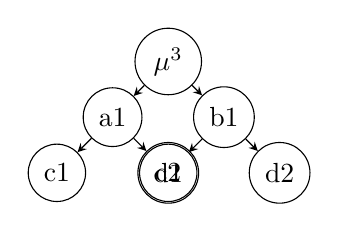
\begin{tikzpicture}[level distance=2cm,
                    level 1/.style={sibling distance=6cm},
                    level 2/.style={sibling distance=3cm}]

    % Root node
    \node [circle, draw] (root)
        {$\mu^3$};

    % Level 1 nodes
    \node [below left of=root, circle, draw] (a1) {a1};
    \node [below right of=root, circle, draw] (b1) {b1};

    % Level 2 nodes
    \node [below left of=a1, circle, draw] (c1) {c1};
    \node [below right of=a1, circle, draw] (d1) {d1};
    \node [below left of=b1, circle, draw] (c2) {c2};
    \node [below right of=b1, circle, draw] (d2) {d2};

    % Draw edges
    \draw[-stealth] (root) -- (a1);
    \draw[-stealth] (root) -- (b1);
    \draw[-stealth] (a1) -- (c1);
    \draw[-stealth] (a1) -- (d1);
    \draw[-stealth] (b1) -- (c2);
    \draw[-stealth] (b1) -- (d2);

\end{tikzpicture}

\end{document}